\documentclass{article}
\usepackage{tikz}
\usepackage[margin=1in]{geometry}

\begin{document}
\thispagestyle{empty}
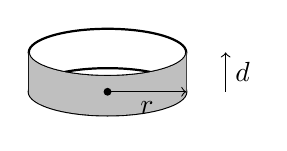
\begin{tikzpicture}
    % Define parameters
    \def\r{1}      % radius
    \def\d{0.5}      % height
    \pgfmathsetmacro{\rminor}{0.3*\r}  % minor axis for 3D effect

    % Draw the cylindrical shell
    % Bottom ellipse (solid - visible edge)
    \draw[thick] (0,0) ellipse ({\r} and {\rminor});

    % Top ellipse (dashed - open top)
    \draw[thick] (0,\d) ellipse ({\r} and {\rminor});

    % Side lines
    \draw[thick] (-\r,0) -- (-\r,\d);
    \draw[thick] (\r,0) -- (\r,\d);

    % Fill the visible curved surface
    \fill[lightgray] (-\r,0) -- (-\r,\d) arc (180:360:{\r} and {\rminor}) -- (\r,0) arc (180:360:{-\r} and {\rminor});

    % Add labels
    % Radius
    \draw[->] (0,0) -- (\r,0);
    \node[below] at (\r/2,0) {$r$};

    % Height
    \draw[->] (\r+0.5,0) -- (\r+0.5,\d);
    \node[right] at (\r+0.5,\d/2) {$d$};

    % Add center point
    \fill (0,0) circle (0.05);
\end{tikzpicture}
\end{document}
